\documentclass[conference]{IEEEtran}

% Settings
\IEEEoverridecommandlockouts
\usepackage{cite}
\usepackage{amsmath,amssymb,amsfonts}
\usepackage{algorithmic}
\usepackage{graphicx}
\usepackage{textcomp}
\usepackage{xcolor}

\graphicspath{ {../images/} }

\def\BibTeX{{\rm B\kern-.05em{\sc i\kern-.025em b}\kern-.08em
    T\kern-.1667em\lower.7ex\hbox{E}\kern-.125emX}}
\begin{document}

% Info

\title{What makes a house high quality?\\ }

\author{
    \IEEEauthorblockN{Barış Deniz Sağlam}
    \IEEEauthorblockA{
        \textit{Informatics Institute} \\
        \textit{Middle East Technical University} \\
        Ankara, Turkey \\
        e155841@metu.edu.tr
    }
}

% Paper

\maketitle

\begin{abstract}
This paper investigates two research questions on Ames Housing Dataset:
\begin{enumerate}
    \item Can we predict overal quality (\textit{OverallQual}) of houses?
    \item Which features are good contributor and predictors of overall quality? 
\end{enumerate}
A random forest regression model is trained for this purpose and Shapley values
are used to explain the trained model. We found that external quality and built year features are
good predictors for overall quality of the house.
\end{abstract}

\begin{IEEEkeywords}
Regression, Random Forest, Model Explainability, Shapley Values, SHAP
\end{IEEEkeywords}

\section{Introduction}

Ames Housing Dataset \cite{DeCock2011} consists of the 2930 house sale records in Ames, Iowa from 2006 to 2021.
With 23 nominal, 23 ordinal, 14 discrete, and 20 continuous variables \cite{DeCock2011}, 
it's a sufficiently rich dataset to experiment with machine learning algorithms.
We investigate two research questions in this paper:
\begin{enumerate}
\item Can we predict overal quality (\textit{OverallQual}) of houses?
\item Which features are good contributors or predictors of overall quality? 
\end{enumerate}
For the first research question, we train and tune linear regression models, and random forest models.
Then, we apply model explainability techniques to understand the contribution of each feature.

\subsection{Literature Search}

Compared to the classical software, machine learning models are much more complex and mostly black boxes. 
However, it's often needed to understand and explain why a machine learning model 
made an inference in production systems. In GDPR, it's required that every individual has 
the right to obtain an explanation for an algorithmic assessment. For example, a
bank is obligated to provide an explanation to a customer for a loan application rejected.
As machine learning models have been gaining popularity in the recent years, explainability
of them have been becoming more important. Hence, many studies have been conducted on model explainability. 
The approaches can be split into two categories \cite{molnar2019}: 
\begin{itemize}
    \item Explainable models
    \item Model-agnostic interpretation methods
\end{itemize}
The first approach is to train explainable models at the first place, such as decision trees. Although this approach
sounds reasonable, it excludes many black-box models that perform well in practice such as
deep learning models. Whereas, with the model agnostic approach, any machine learning model
can be explained with various techniques proposed. 

Model agnostic methods can be further split into two categories: global and local 
explainers. Local explanation methods are capable of providing an explanation for
any data instance. Whereas, global explanation methods provide a single explanation 
for the model such feature importances.

One of the main global model explanation methods is permutation 
feature importance method introduced by Breiman (2001) \cite{Breiman2001} for random forest models and made model agnostic by
Fisher, Rudin, and Dominici (2019) \cite{Fisher2019}. The method estimates feature importances in a trained model 
with such an algorithm \cite{molnar2019}:
\begin{enumerate}
    \item Estimate the model error with the original dataset.
    \item For each feature \textbf{\textit{j}}, permute the values in the feature and 
    estimate the model error with the predictions made with this modified data. 
    The importance of the feature \textbf{\textit{j}}, is the difference between the new error and 
    the original error. 
\end{enumerate}
Intuitively, when a feature is important for the model, model performance degrades
when the values of that feature is permuted. 

A well-known local model-agnostic explanation method is Shapley value method, introduced by
by Shapley (1953) \cite{shapley1953value} as a technique for coalitional game theory. It estimates 
individual player's performance when the game is not individualistic. The method
achieves this by measuring the performances of the different coalitions of
players. The idea is that if a player performs well, the coalitions, i.e. teams, 
that contain the player also should perform well. The method is applied in machine learning
by treating the features as the players and the model inference as the game. It
forms different sets of features and measures the model performance. Then, for each feature, 
it averages all the scores of the feature set the feature was included. Since the method can be
applied to both a single data point and a full dataset, it can generate both local and global 
explanations. 
A useful property of Shapley values is that they are additive such that their summation is equal to the model's prediction for a data point. 
The asymptotic runtime of original Shapley algorithm is exponential with the number of features, hence, it's too slow. 
Lundberg and Lee (2017) \cite{Lundberg2017} proposed a variation of the method, SHAP, with polynomial time for tree-based models.

\section{Methods}

\subsection{Data quality}

Before analyzing the dataset, we inspect the description of the dataset to identify each variable's data type and split them into three types: numerical, ordinal, and nominal. The data type of a variable is important when choosing encoding and imputation methods for that variable. 
We also determine the order of categories for ordinal variables whose order cannot be inferred by \textit{pandas} library \cite{pandas}.
We perform basic data quality checks on variables to ensure that there're no inconsistent values according to the definition of each variable. For instance,
\begin{itemize}
    \item Any date variable cannot be negative.
    \item Month cannot be out of range [1,12].
    \item Area cannot be negative.
    \item The sale year must be greater or equal to all dates related the building such as house built year, garage built year.
\end{itemize}
Any inconsistent value is treated as missing and erased from the dataset.

There are varying number of missing values for variables in the dataset.
Any row in the training dataset which misses the target variable (\textit{OverallQual}) 
is dropped since it cannot be used for training.
For the majority of the categorical variables, there is a category defined representing
missing value (\textit{NA} or \textit{None}) in the description of the dataset.
The missing values in those categorical variables are filled with the corresponding missing 
value defined. After imputing the missing values in such categorical variables, there are
two variables left in the training set that have missing values: \textit{LotFrontage} and \textit{MasVnrArea}.
From Fig.~\ref{fig:missing-heatmap}, it's inferred that the missingness mechanisms 
for both variable are MCAR since there is no correlation between their missingness.
\begin{figure}[htbp]
    \centerline{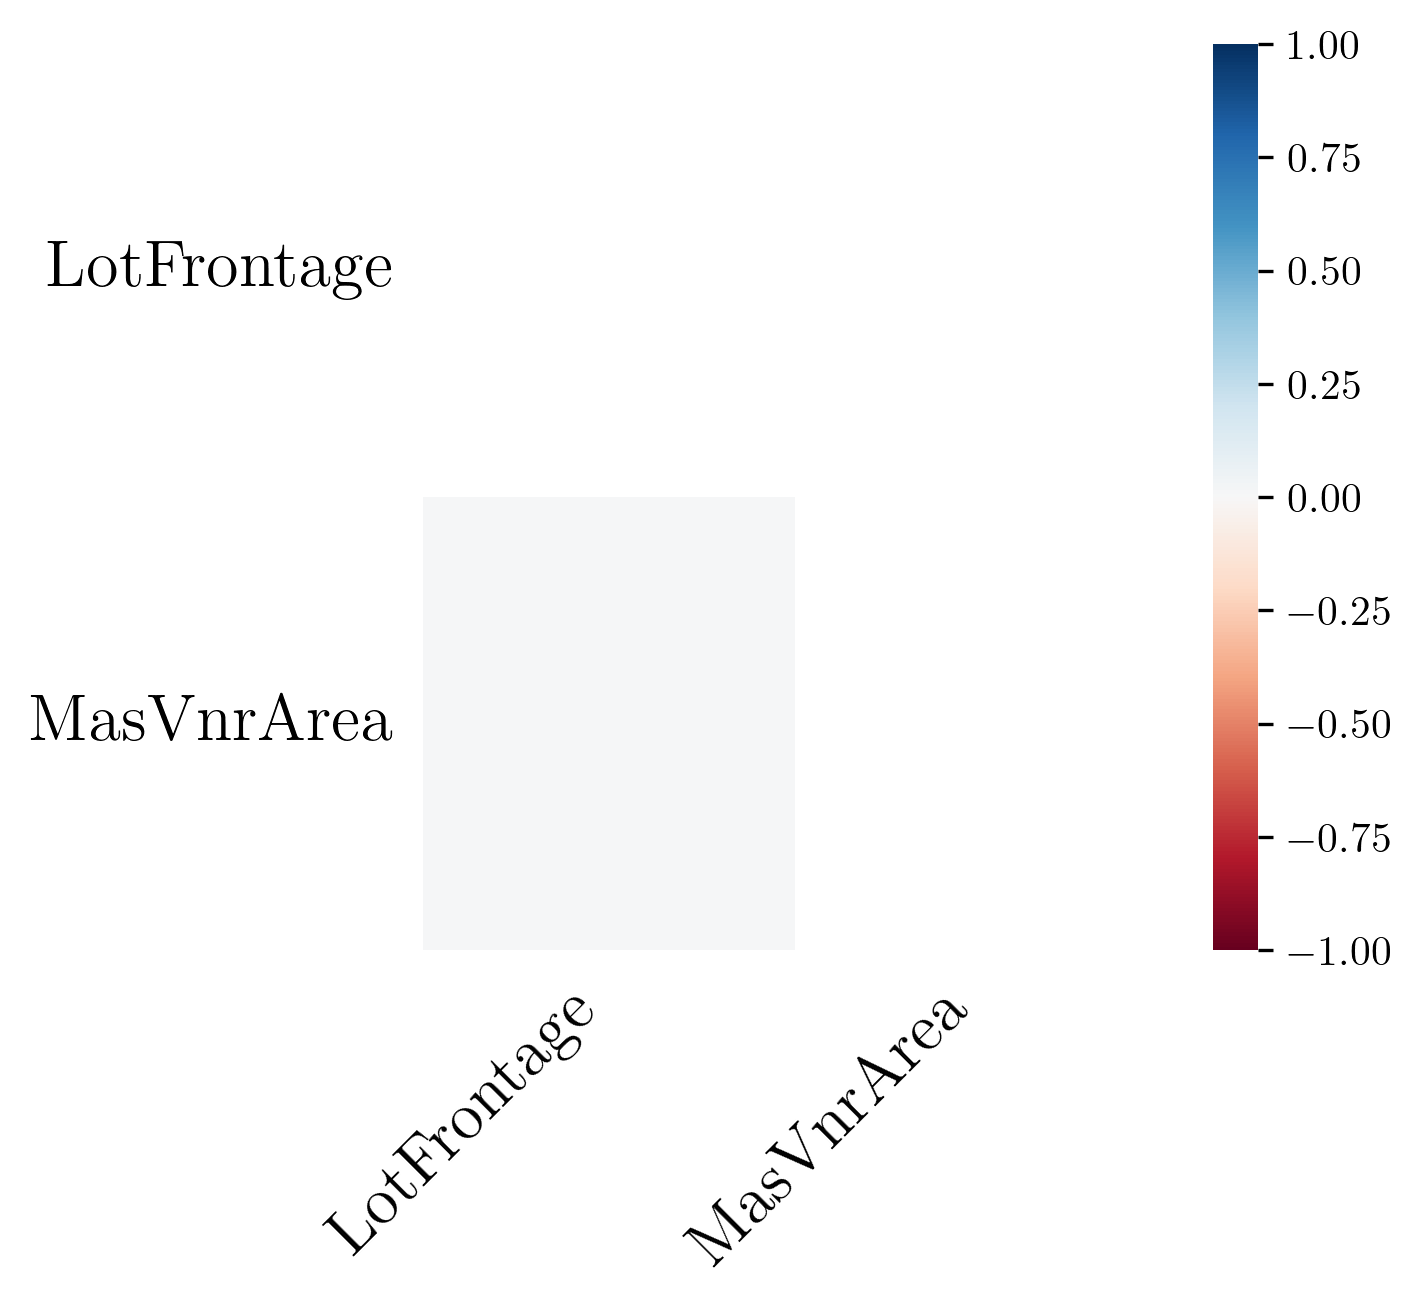
\includegraphics[width = 0.4 \textwidth]{missingno-heatmap.png}}
    \caption{missingno \cite{Bilogur2018} heatmap for missing values}
    \label{fig:missing-heatmap}
\end{figure}
When there is no category defined for missing value, the most frequent value is 
used to impute missing values in the categorical variables.
For numerical variables, the mean imputation is used.

As it's seen from Fig.~\ref{fig:numericals-histogram} and Fig.~\ref{fig:numericals-skewness-bar}, 
while \textit{FullBath}, \textit{GarageArea}, \textit{GarageCars}, and \textit{TotRmsAbvGrd} 
have roughly symmetrical distributions, the rest of the numerical variables are skewed.
\begin{figure}[htbp]
    \centerline{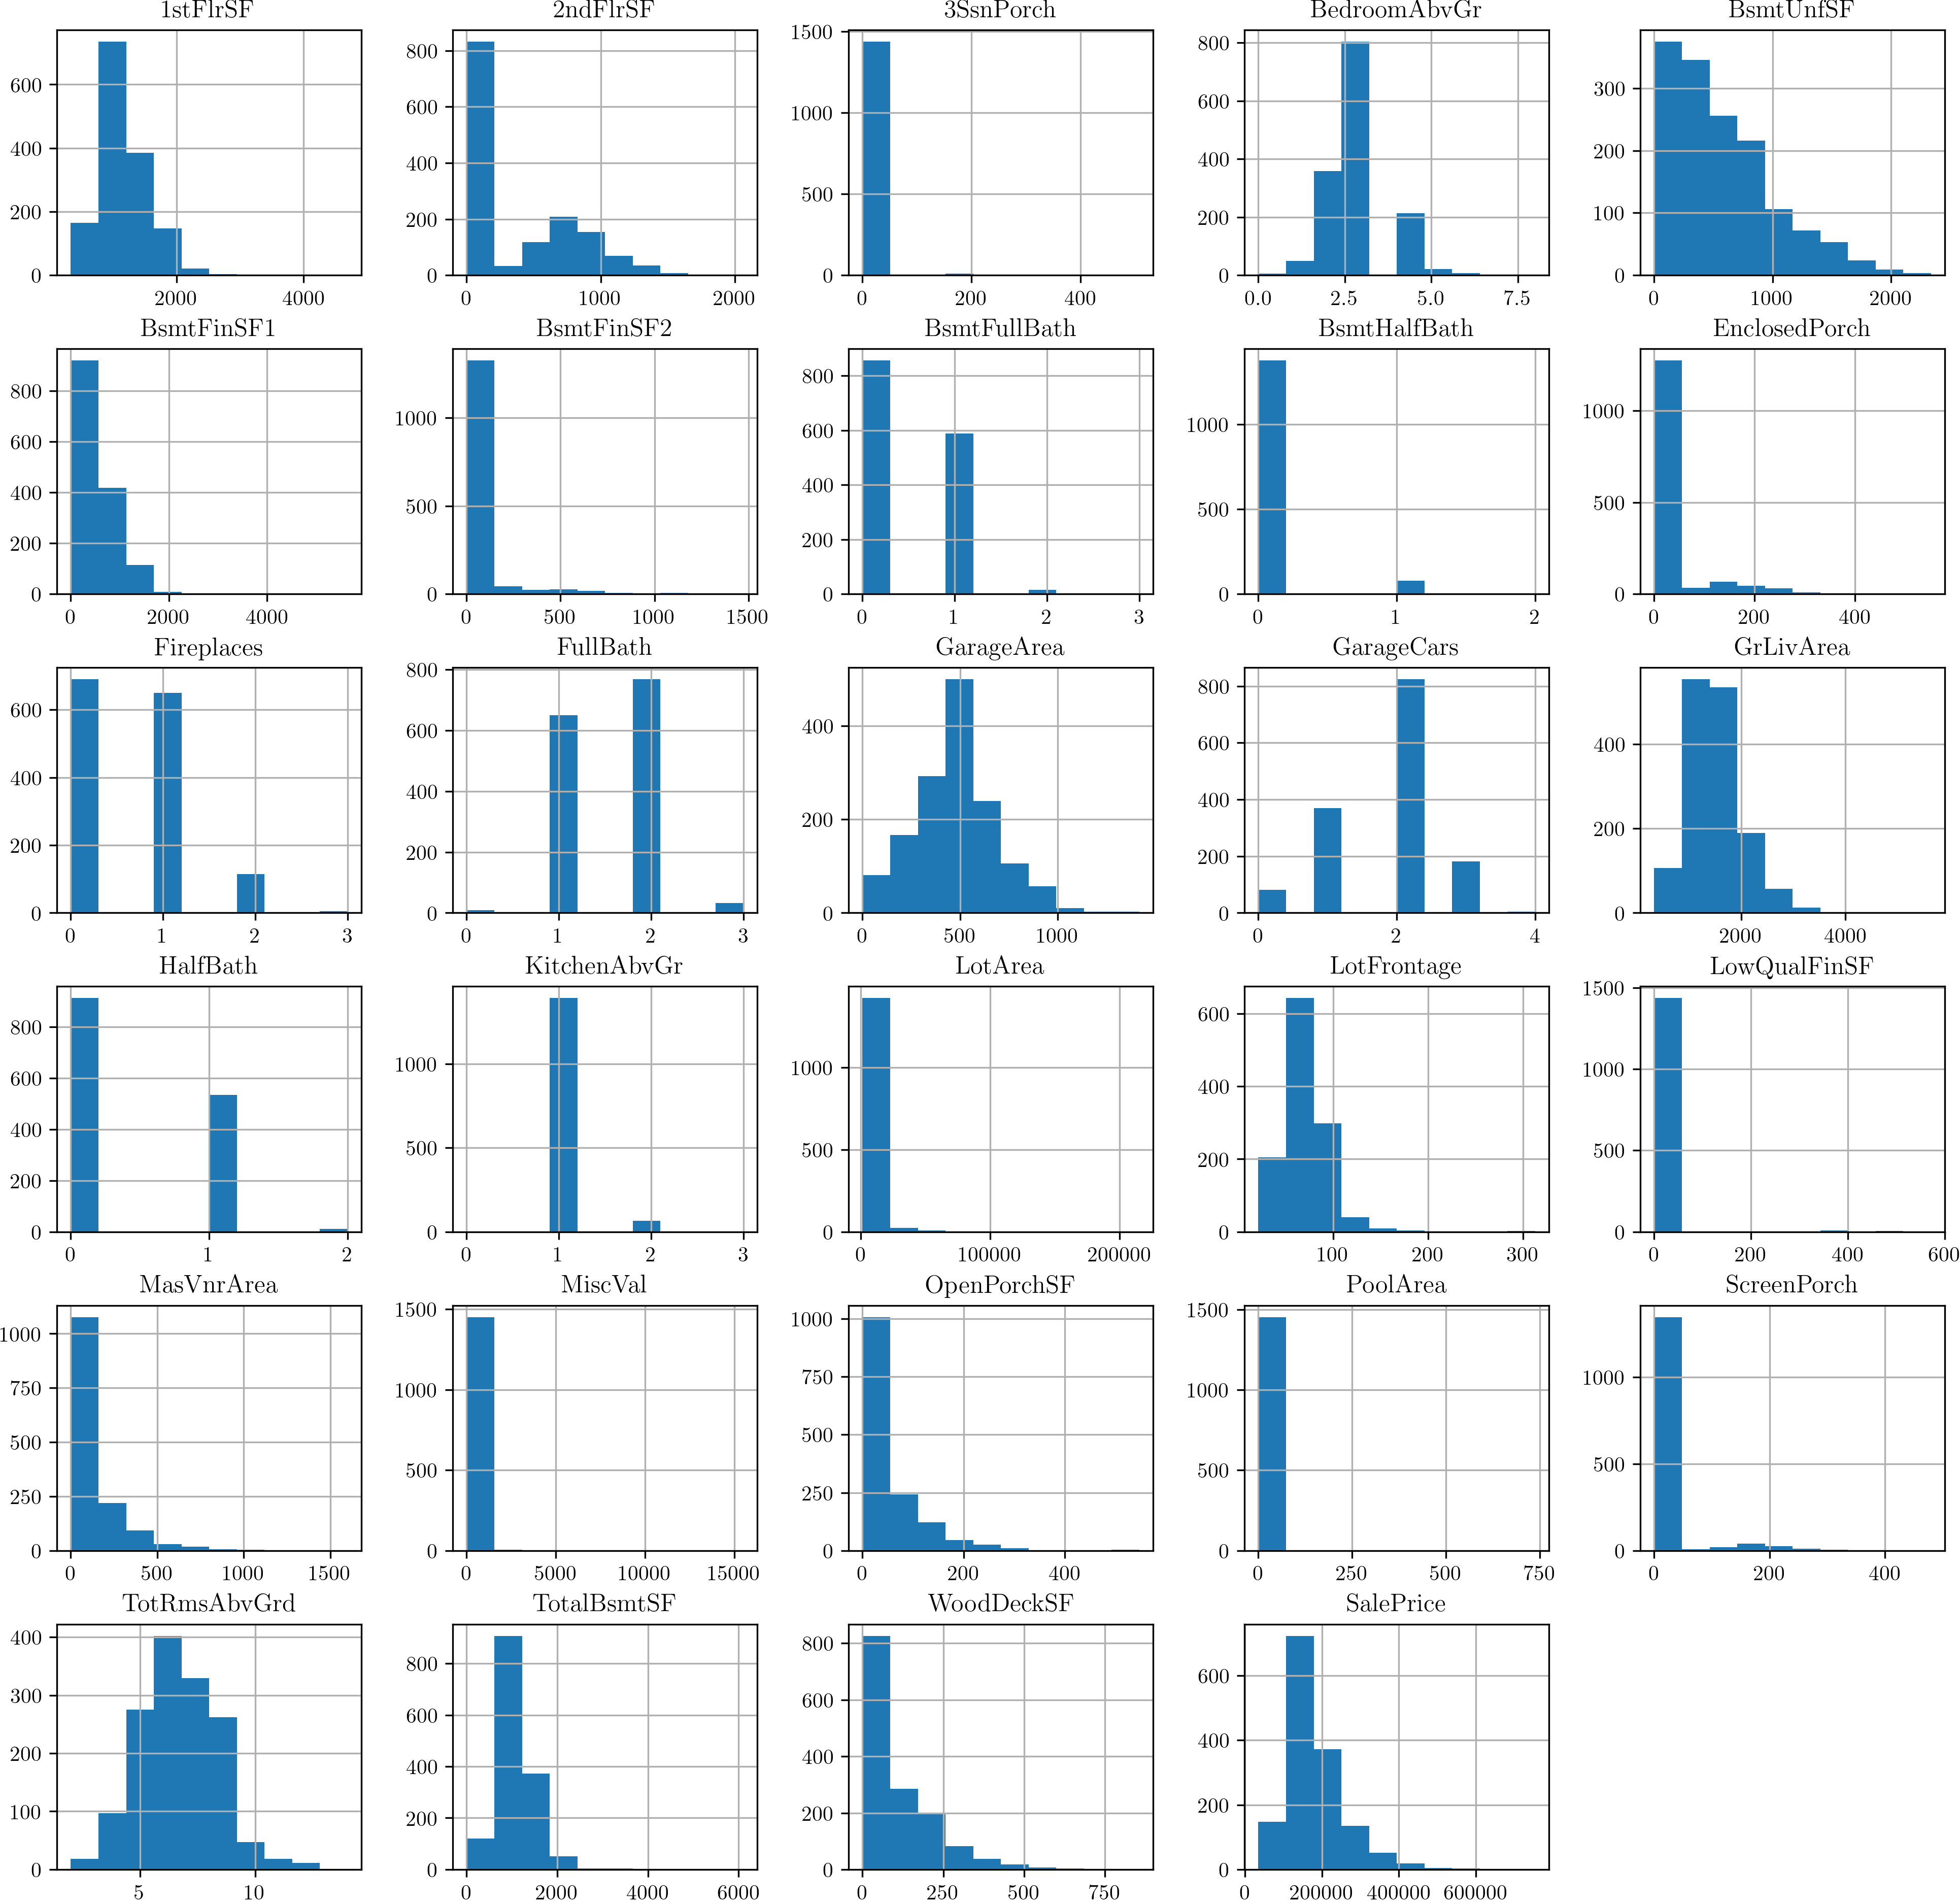
\includegraphics[width = 0.5 \textwidth]{numericals-histogram.png}}
    \caption{Histogram of numerical variables}
    \label{fig:numericals-histogram}
\end{figure}
\begin{figure}[htbp]
    \centerline{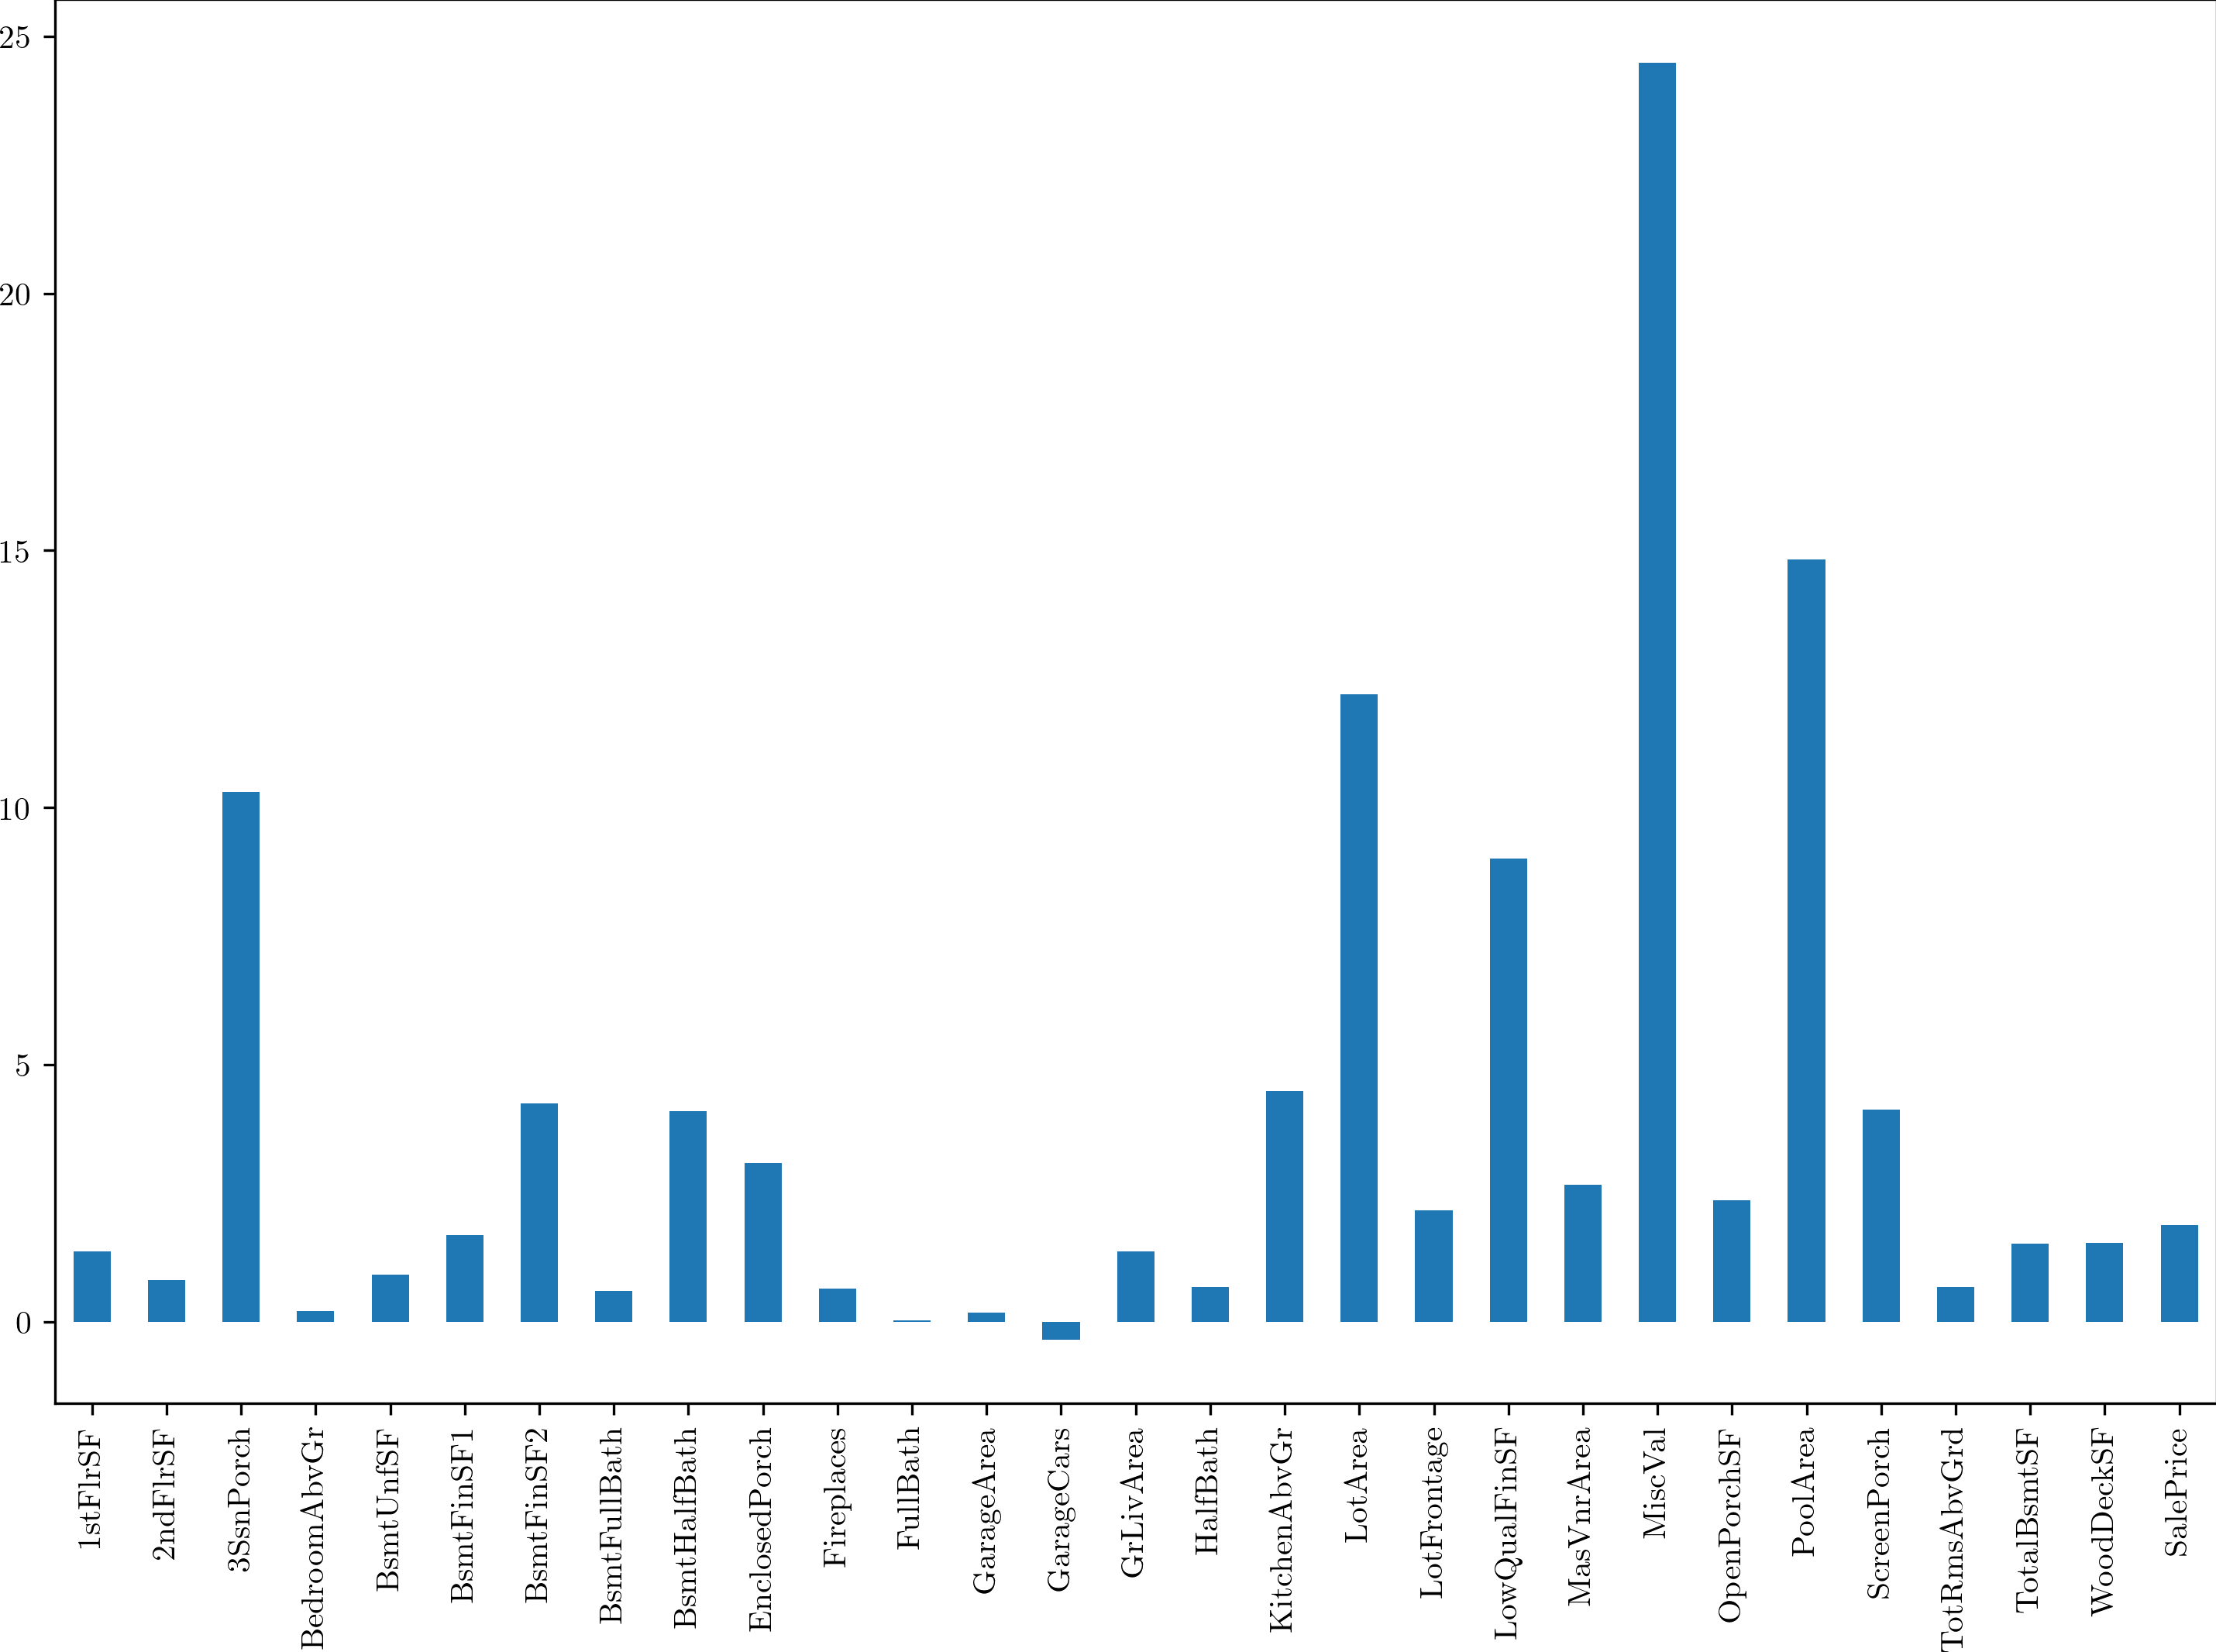
\includegraphics[width = 0.5 \textwidth]{numericals-skewness-bar.png}}
    \caption{Skewness of numerical variables}
    \label{fig:numericals-skewness-bar}
\end{figure}
The numerical variables are scaled to eliminate scale differences among variables.
The numerical variables with symmetrical distribution, 
i.e. the ones with skewness value less than 0.5, are standardized. 
Whereas, the numerical variables with skewed distribution, i.e. with skewness value greater than 0.5, are scaled with min-max scaling.

In all preprocessing steps, only the statistical features of training set are used to 
prevent information leakage from training to evaluation.

\subsection{Dimensionality reduction and feature selection}

Since the target variable is \textit{OverallQual}, 
we remove \textit{SalePrice} and \textit{SaleCondition} features from the dataset to prevent information leakage.
Similarly, we ignore \textit{YrSold} and \textit{MoSold} featuers since the model's predictions should be independent of the sale date.

To achieve a smaller and simpler model, we apply dimensionality reduction and feature selection on the dataset.
For numerical variables, principal component analysis is performed and 
as it's seen from the Fig.~\ref{fig:pca-cumulative-explained-variance},
3 components cover ~90\% of the variance in the numerical variables of dataset. 
Hence, we reduce the all numerical variables to 3 dimension.
\begin{figure}[htbp]
    \centerline{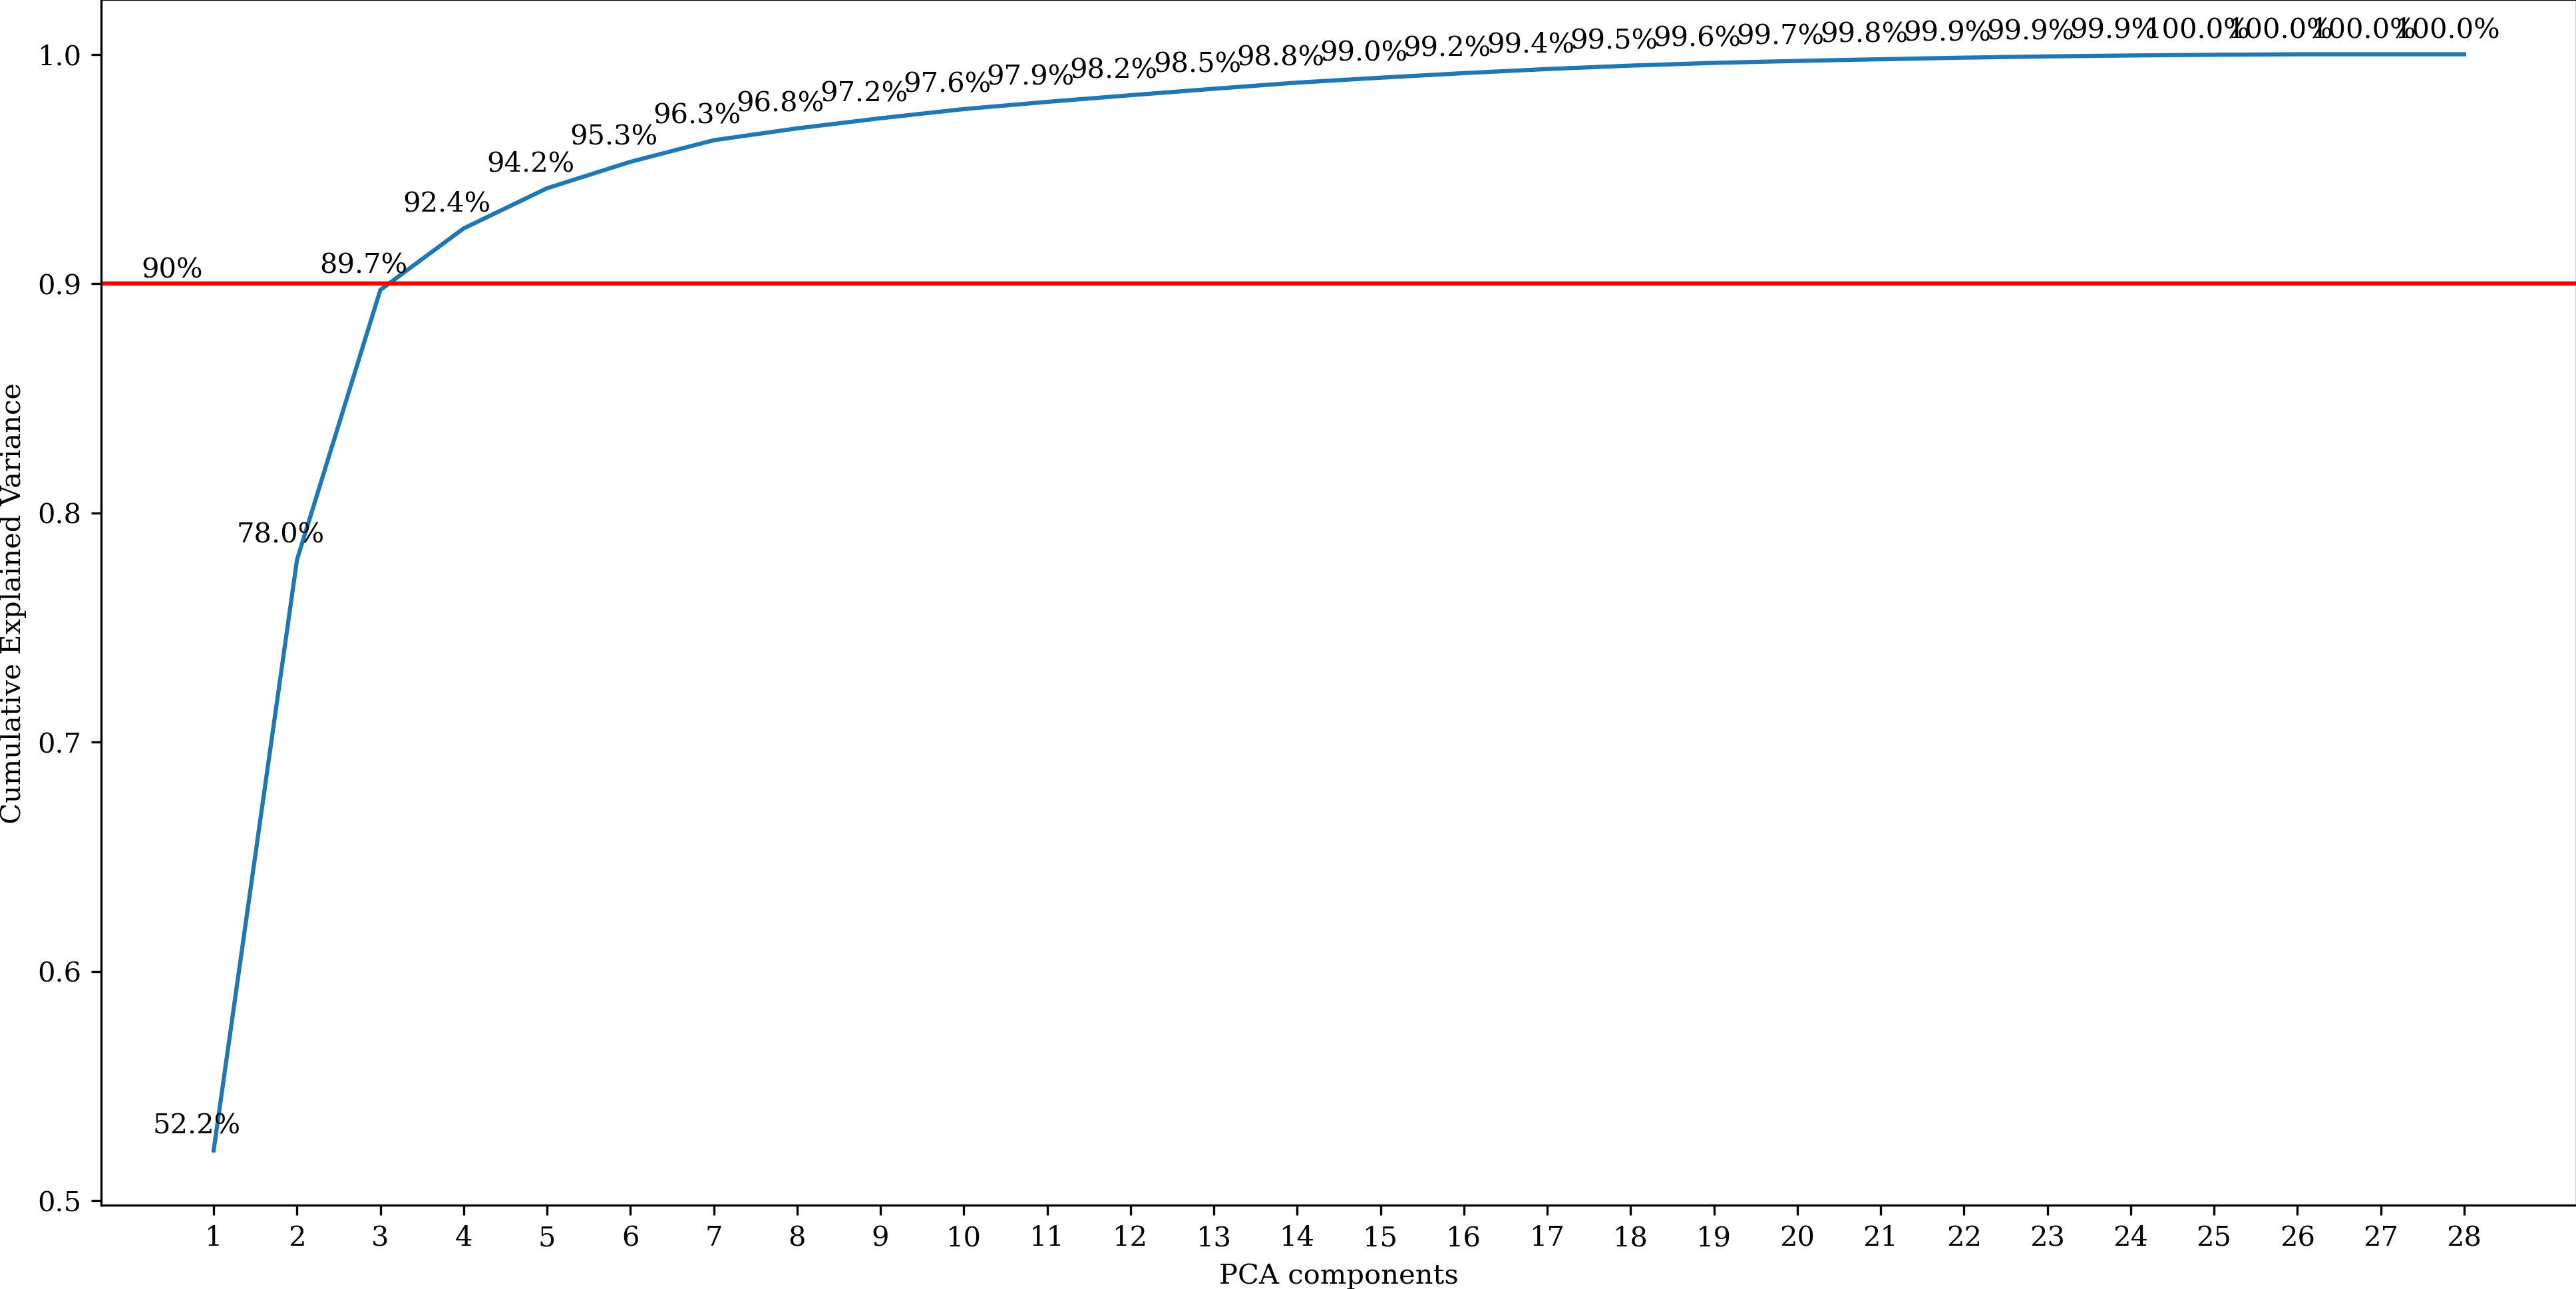
\includegraphics[width = 0.5 \textwidth]{pca-cumulative-explained-variance.png}}
    \caption{PCA - Cumulate Explained Variance}
    \label{fig:pca-cumulative-explained-variance}
\end{figure}

Similarly, for ordinal and nominal variables, we calculate global feature importances with SHAP method. 
We use TreeExplainer from \textit{shap} library \cite{tree-explainer} on the trained model with the validation dataset
to compute Shapley values per data point per feature. Then, we calculate global feature 
importances by taking absolute mean of Shapley values per feature across all data points.
As it's seen from Fig.~\ref{fig:shap-cumulative-feature-importance}, 17 categorical features cover 
90\% of the contributions of all categorical features.
\begin{figure}[htbp]
    \centerline{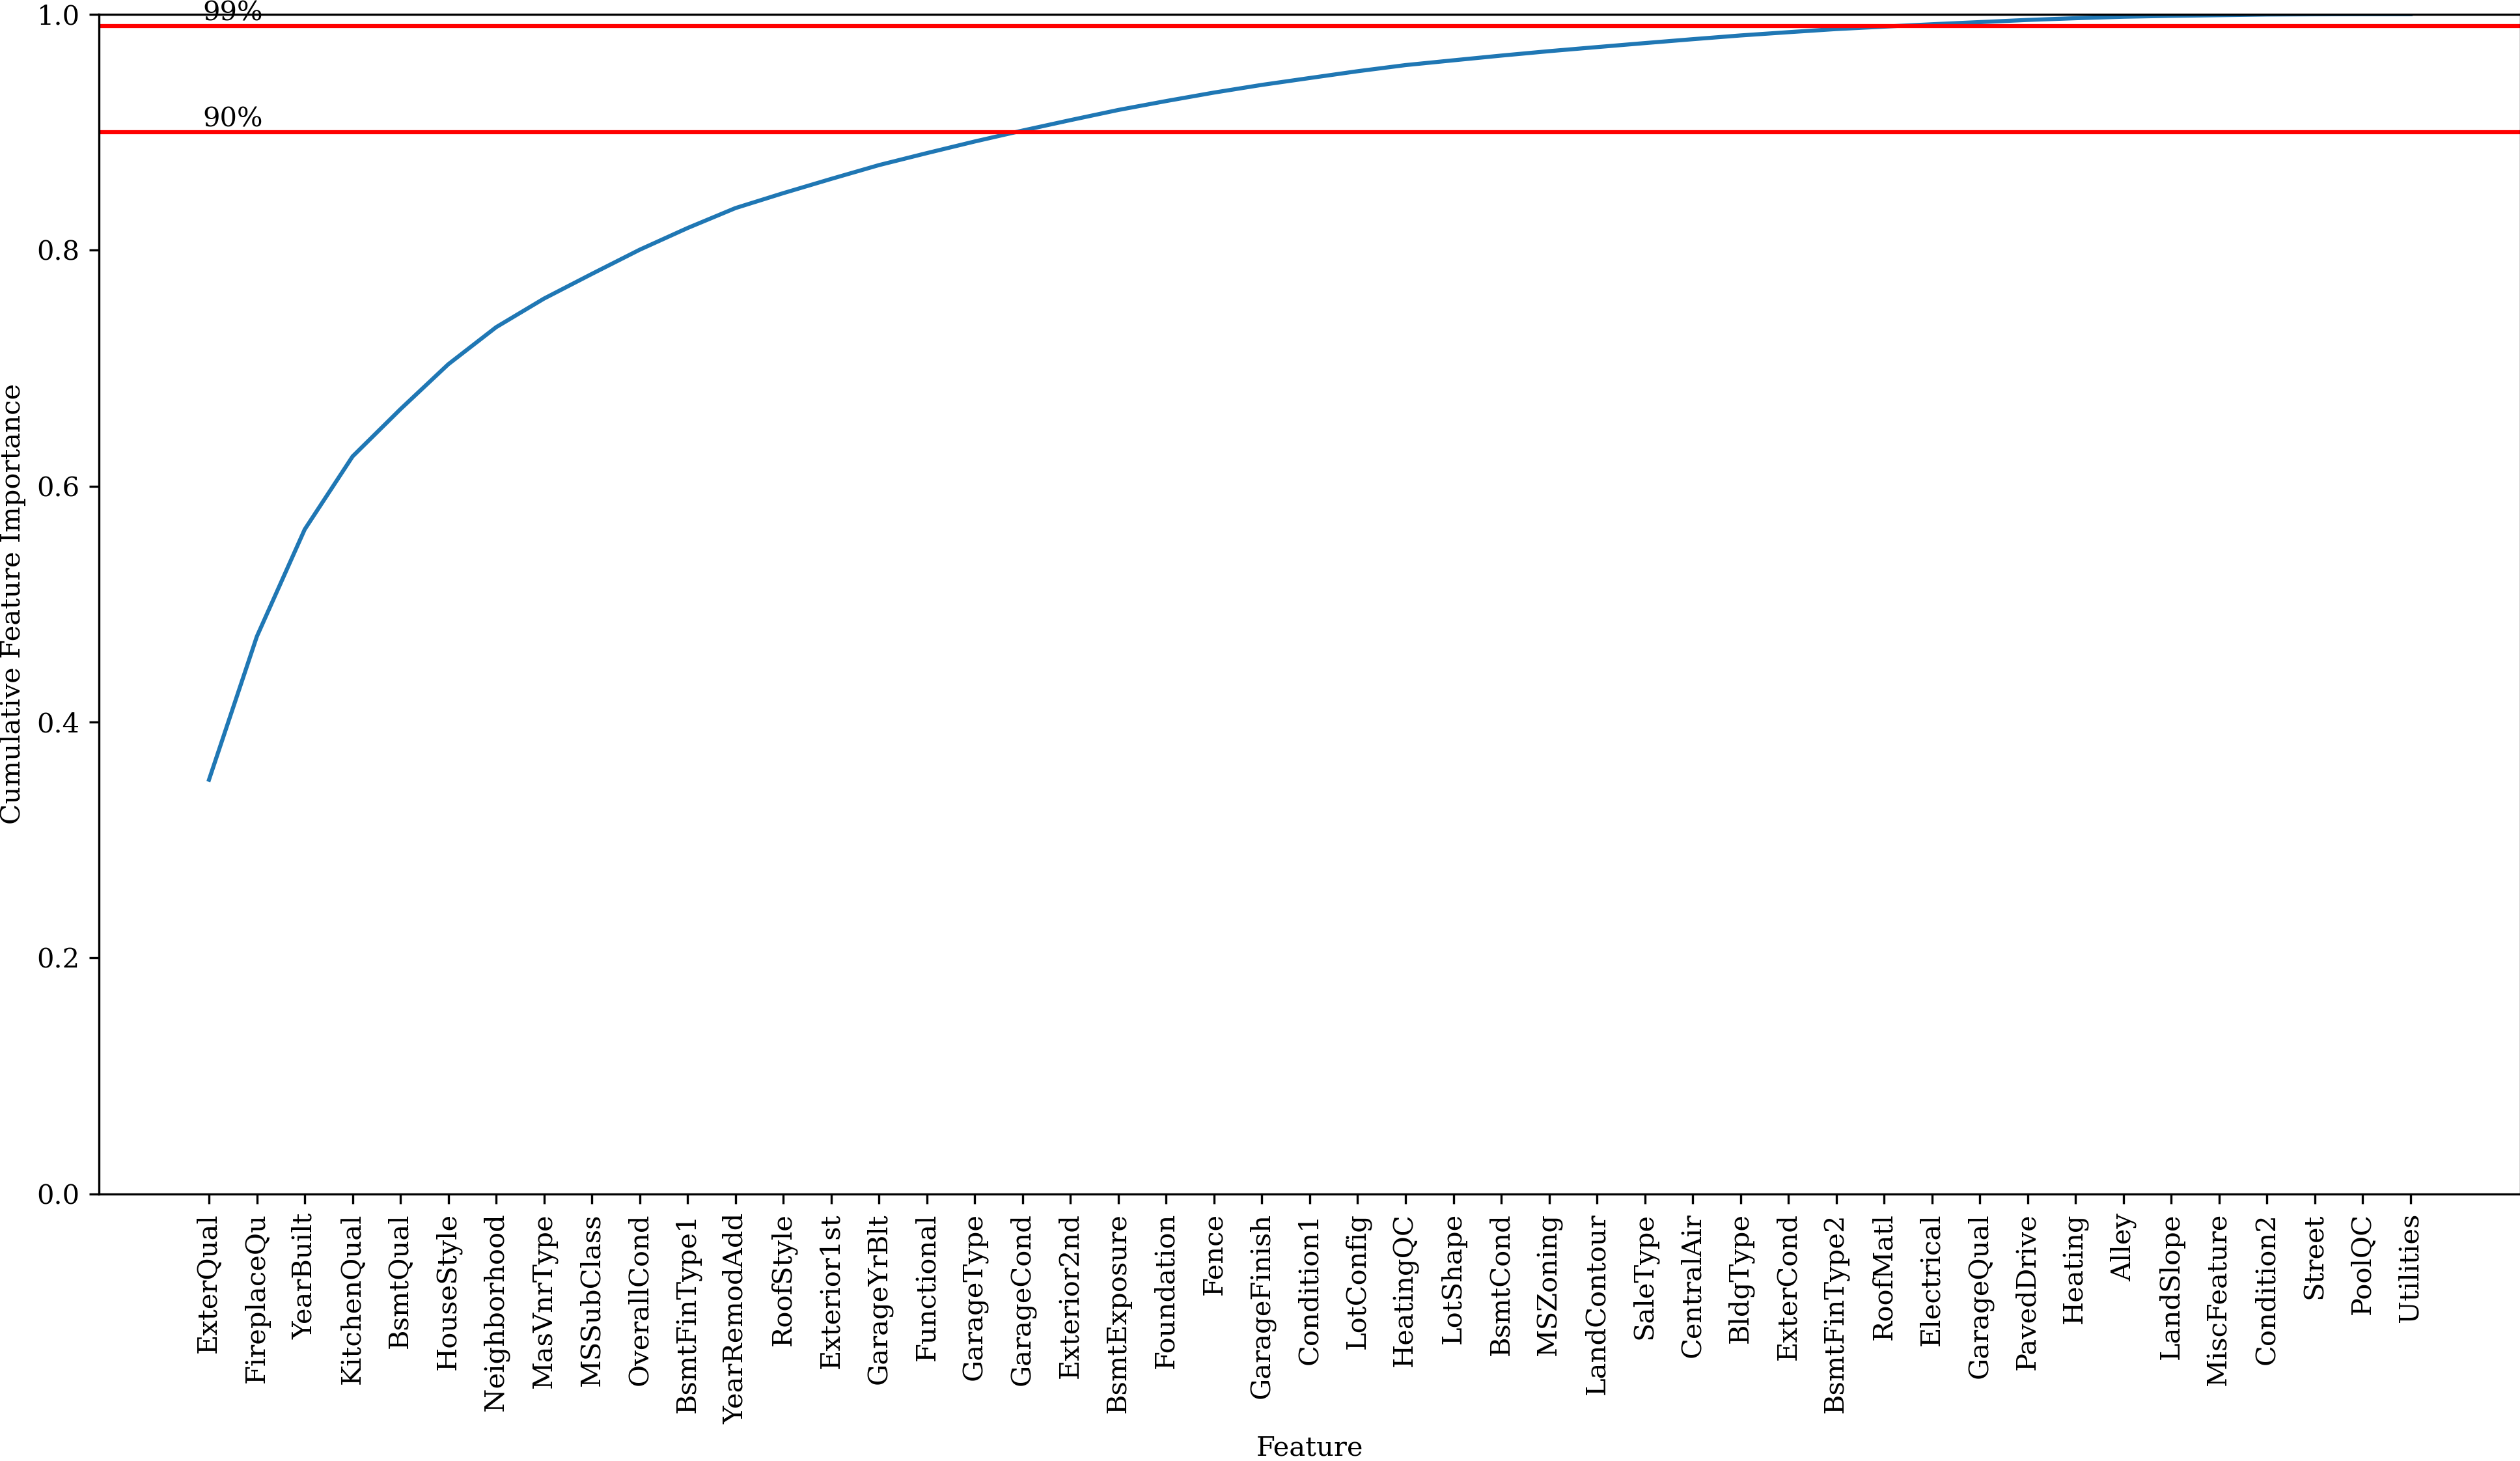
\includegraphics[width = 0.5 \textwidth]{shap-cumulative-feature-importance.png}}
    \caption{SHAP - Cumulative global feature importance}
    \label{fig:shap-cumulative-feature-importance}
\end{figure}

Therefore, we only use the most important ones of the categorical variables 
listed in Table~\ref{table:shap-global-feature-importance} to train our model.
\begin{table}[htbp]
    \caption{SHAP - Global Feature Importance}
\begin{center}
\begin{tabular}{lr}
    \hline
        variable &  \% feature importance \\
    \hline
       ExterQual &    0.288264 \\
       YearBuilt &    0.188572 \\
     FireplaceQu &    0.139039 \\
     KitchenQual &    0.035111 \\
        BsmtQual &    0.033722 \\
      HouseStyle &    0.032869 \\
    Neighborhood &    0.031666 \\
     OverallCond &    0.020790 \\
      MasVnrType &    0.020446 \\
    BsmtFinType1 &    0.019180 \\
      MSSubClass &    0.019014 \\
       RoofStyle &    0.014213 \\
     Exterior1st &    0.013521 \\
    YearRemodAdd &    0.012969 \\
      GarageType &    0.010599 \\
     GarageYrBlt &    0.009502 \\
      Foundation &    0.008329 \\
    \hline
\end{tabular}
\label{table:shap-global-feature-importance}
\end{center}
\end{table}

\subsection{Model training and evaluation}

The dataset is split into train and validation sets with 80:20 ratio. 
The test set is not used for training or model selection.

A random forest model is a collection of decision trees under the hood. 
It averages the predictions of all decision trees to make a prediction. 
This reduces the variance in the model error.
We train random forest models with 5-fold cross validation and grid search of 
hyper-parameter space with \textit{scikit-learn} library \cite{scikit-learn}. 
Due to constraints on the computation resources available for the research, 
18 different hyper-parameter configurations are used for random forest regressor. 
We also train a linear regression model as a baseline. 
R2 and mean squared error metrics are used to evaluate and compare models' performances during training. 

R2 metric is defined as 

\begin{equation}
    R^2(y, \hat{y}) = 1 - \frac{\sum_{i=1}^{n} (y_i - \hat{y}_i)^2}{\sum_{i=1}^{n} (y_i - \bar{y})^2} \label{eq:r2}
\end{equation}

Hence, R2 score is:
\begin{itemize}
    \item 1 for a perfect model, always predicting the correct value
    \item 0 for a regression model that always predicts the sample mean
    \item negative for worse models
\end{itemize}
Hence, R2 score is a well-suited metric for regression problems. 

The random forest regressor clearly outperforms linear regressor 
by achieving 0.743 R2 score and 0.412 MSE on the validation set.

\begin{table}[htbp]
    \caption{Model scores on train and validation sets}
\begin{center}
\begin{tabular}{lrrr}
    \hline
    {Model} & Set &  R2 (higher is better) &  MSE (lower is better) \\
    \hline
    Random Forest    & Train set      & 0.945 & 0.087 \\
                     & Validation set & 0.734 & 0.412 \\
    Linear Regressor & Train set      & 0.665 & 0.562 \\
                     & Validation set & 0.564 & 0.750 \\
    \hline
\end{tabular}
\label{table:model-scores}
\end{center}
\end{table}

\subsection{Model explanation}

Shap method provides local explanations to data points as well. It's possible 
to explain a model's prediction for a data point with Shapley values. 
A SHAP feature contribution graph starts from the 
expected value for prediction and builds up the prediction by adding each feature's
contribution.
For example, for the data point with OverallQual=10, 
the contribution of each feature can be seen from the Fig.~\ref{fig:shap-local-10}.
A high external quality and a late built year features make most contribution for this house's overall quality. 
\begin{figure}[htbp]
    \centerline{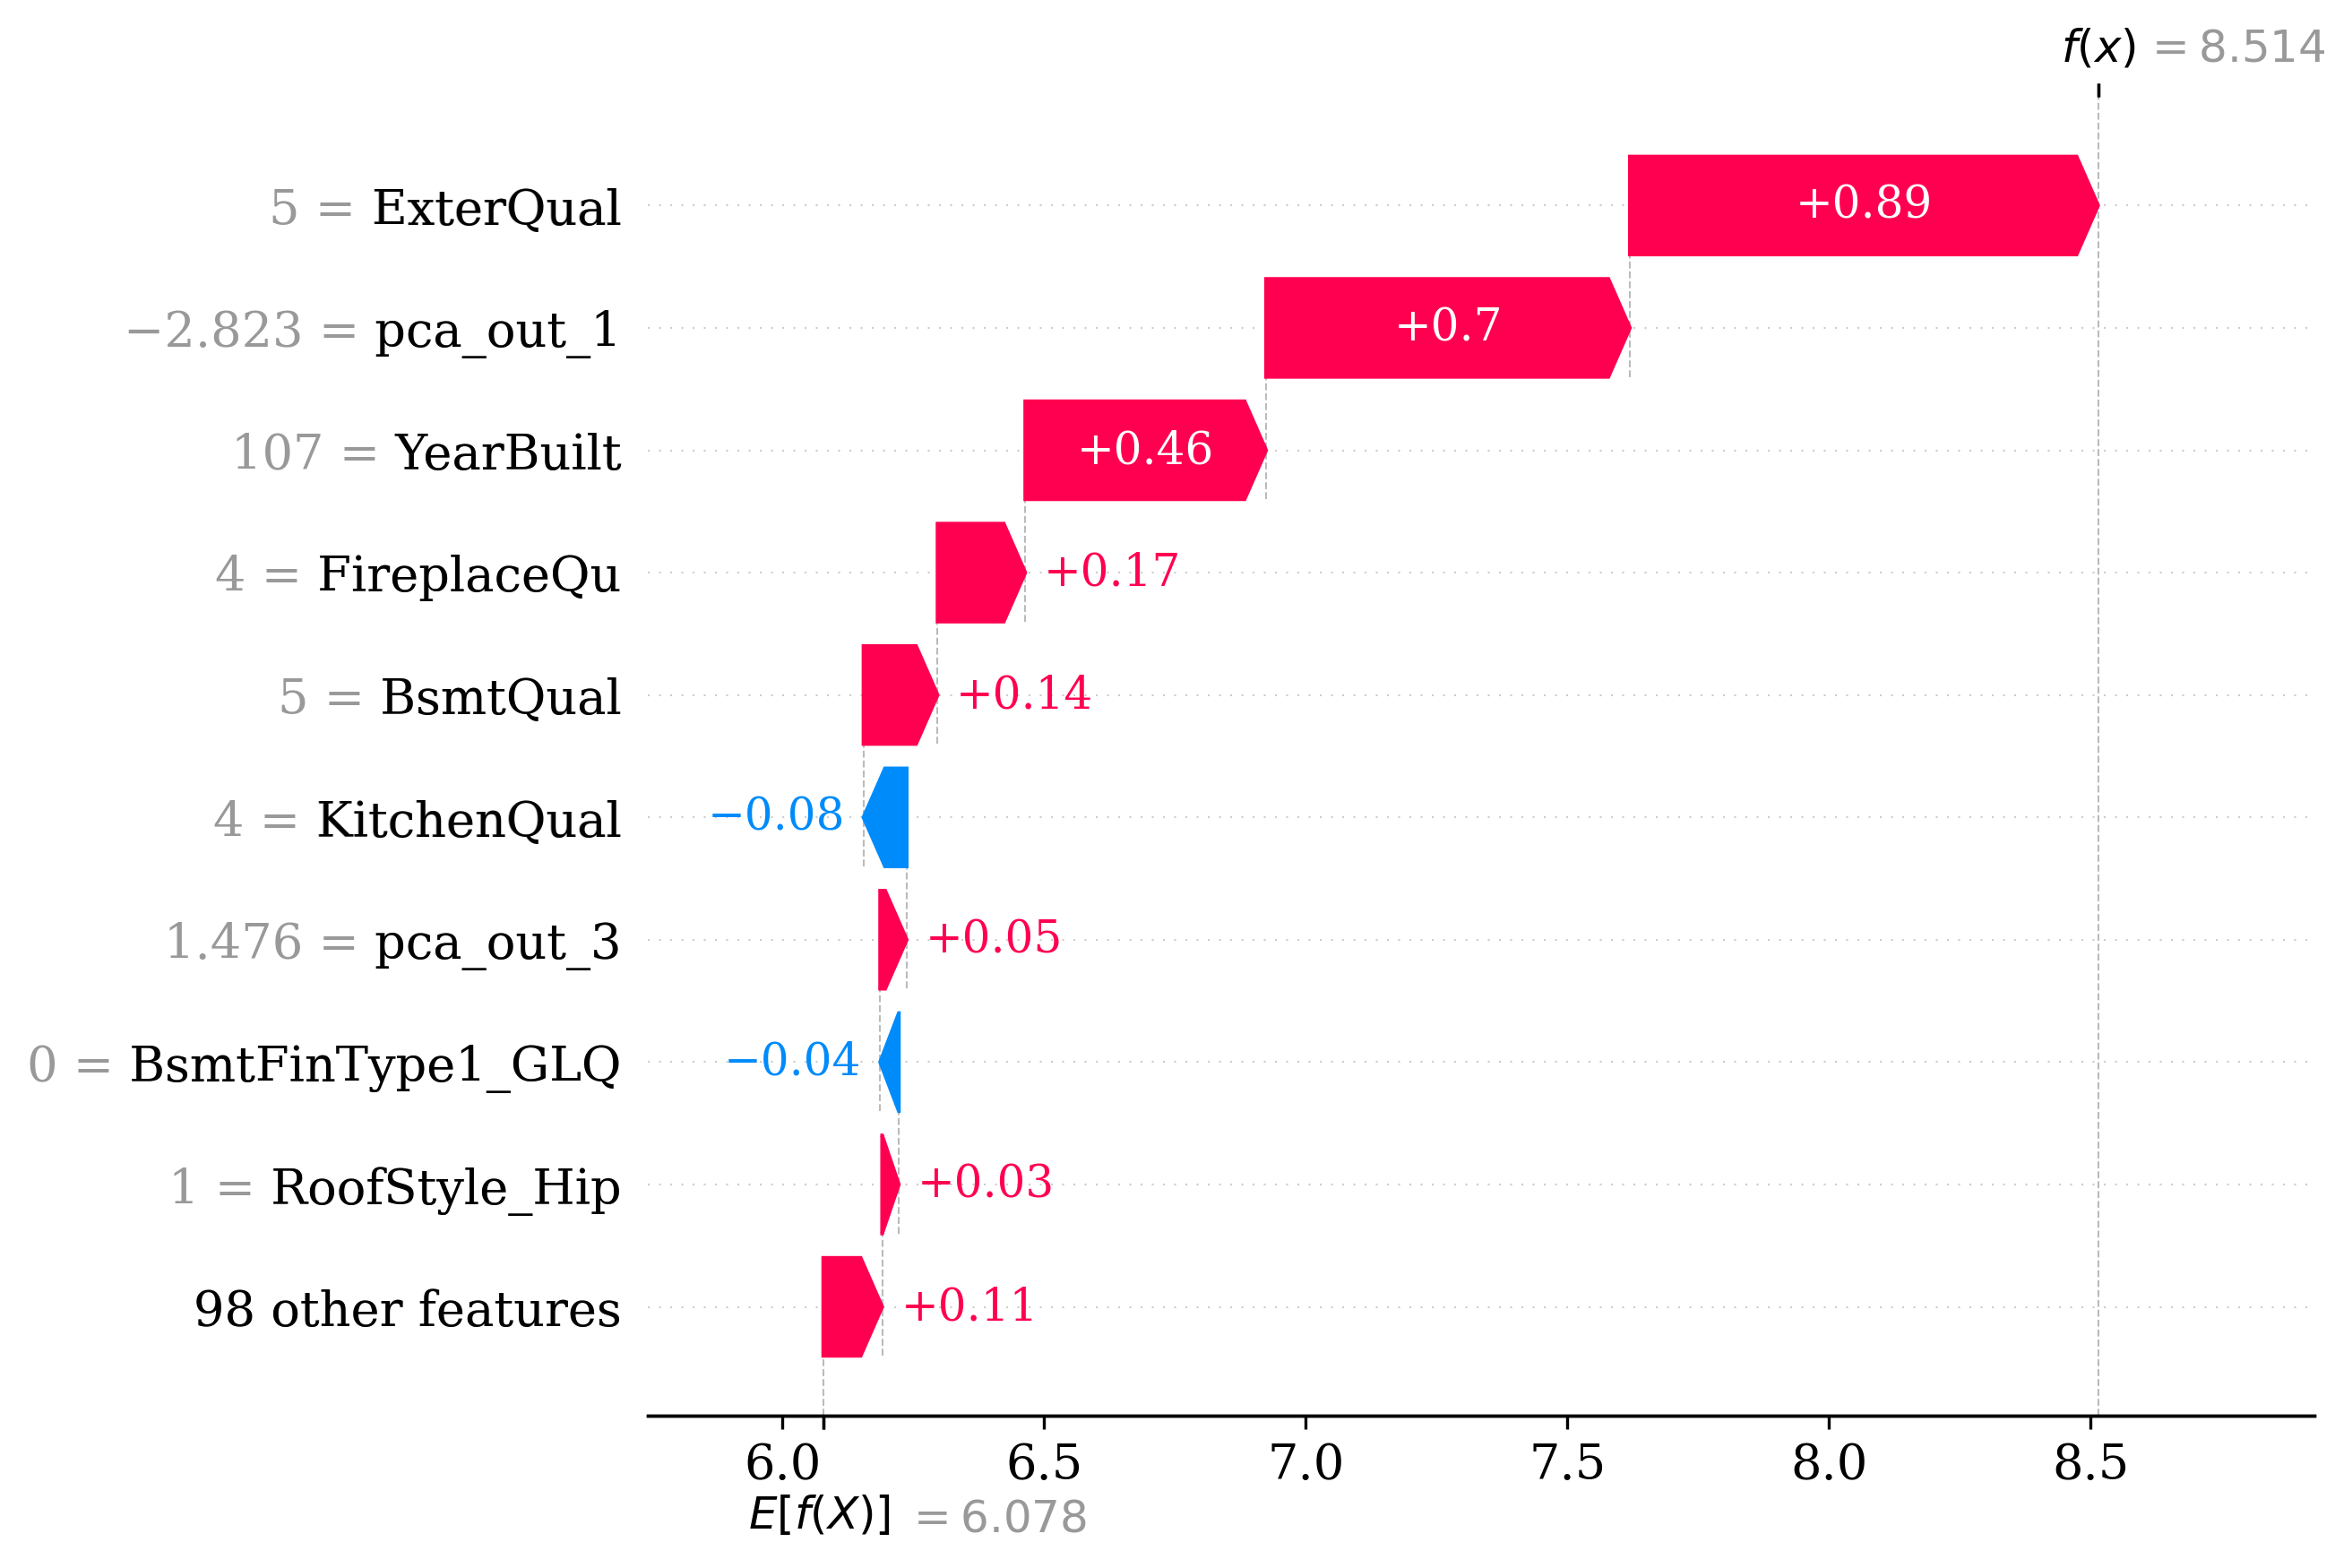
\includegraphics[width = 0.5 \textwidth]{shap-local-10.png}}
    \caption{SHAP - Feature contributions to the prediction}
    \label{fig:shap-local-10}
\end{figure}

Similarly, for the data point with OverallQual=3, 
the contribution of each feature can be seen from the Fig.~\ref{fig:shap-local-3}.
Low external quality, fireplace quality, overall condition, and being an old building 
contributes negatively to overall quality.
\begin{figure}[htbp]
    \centerline{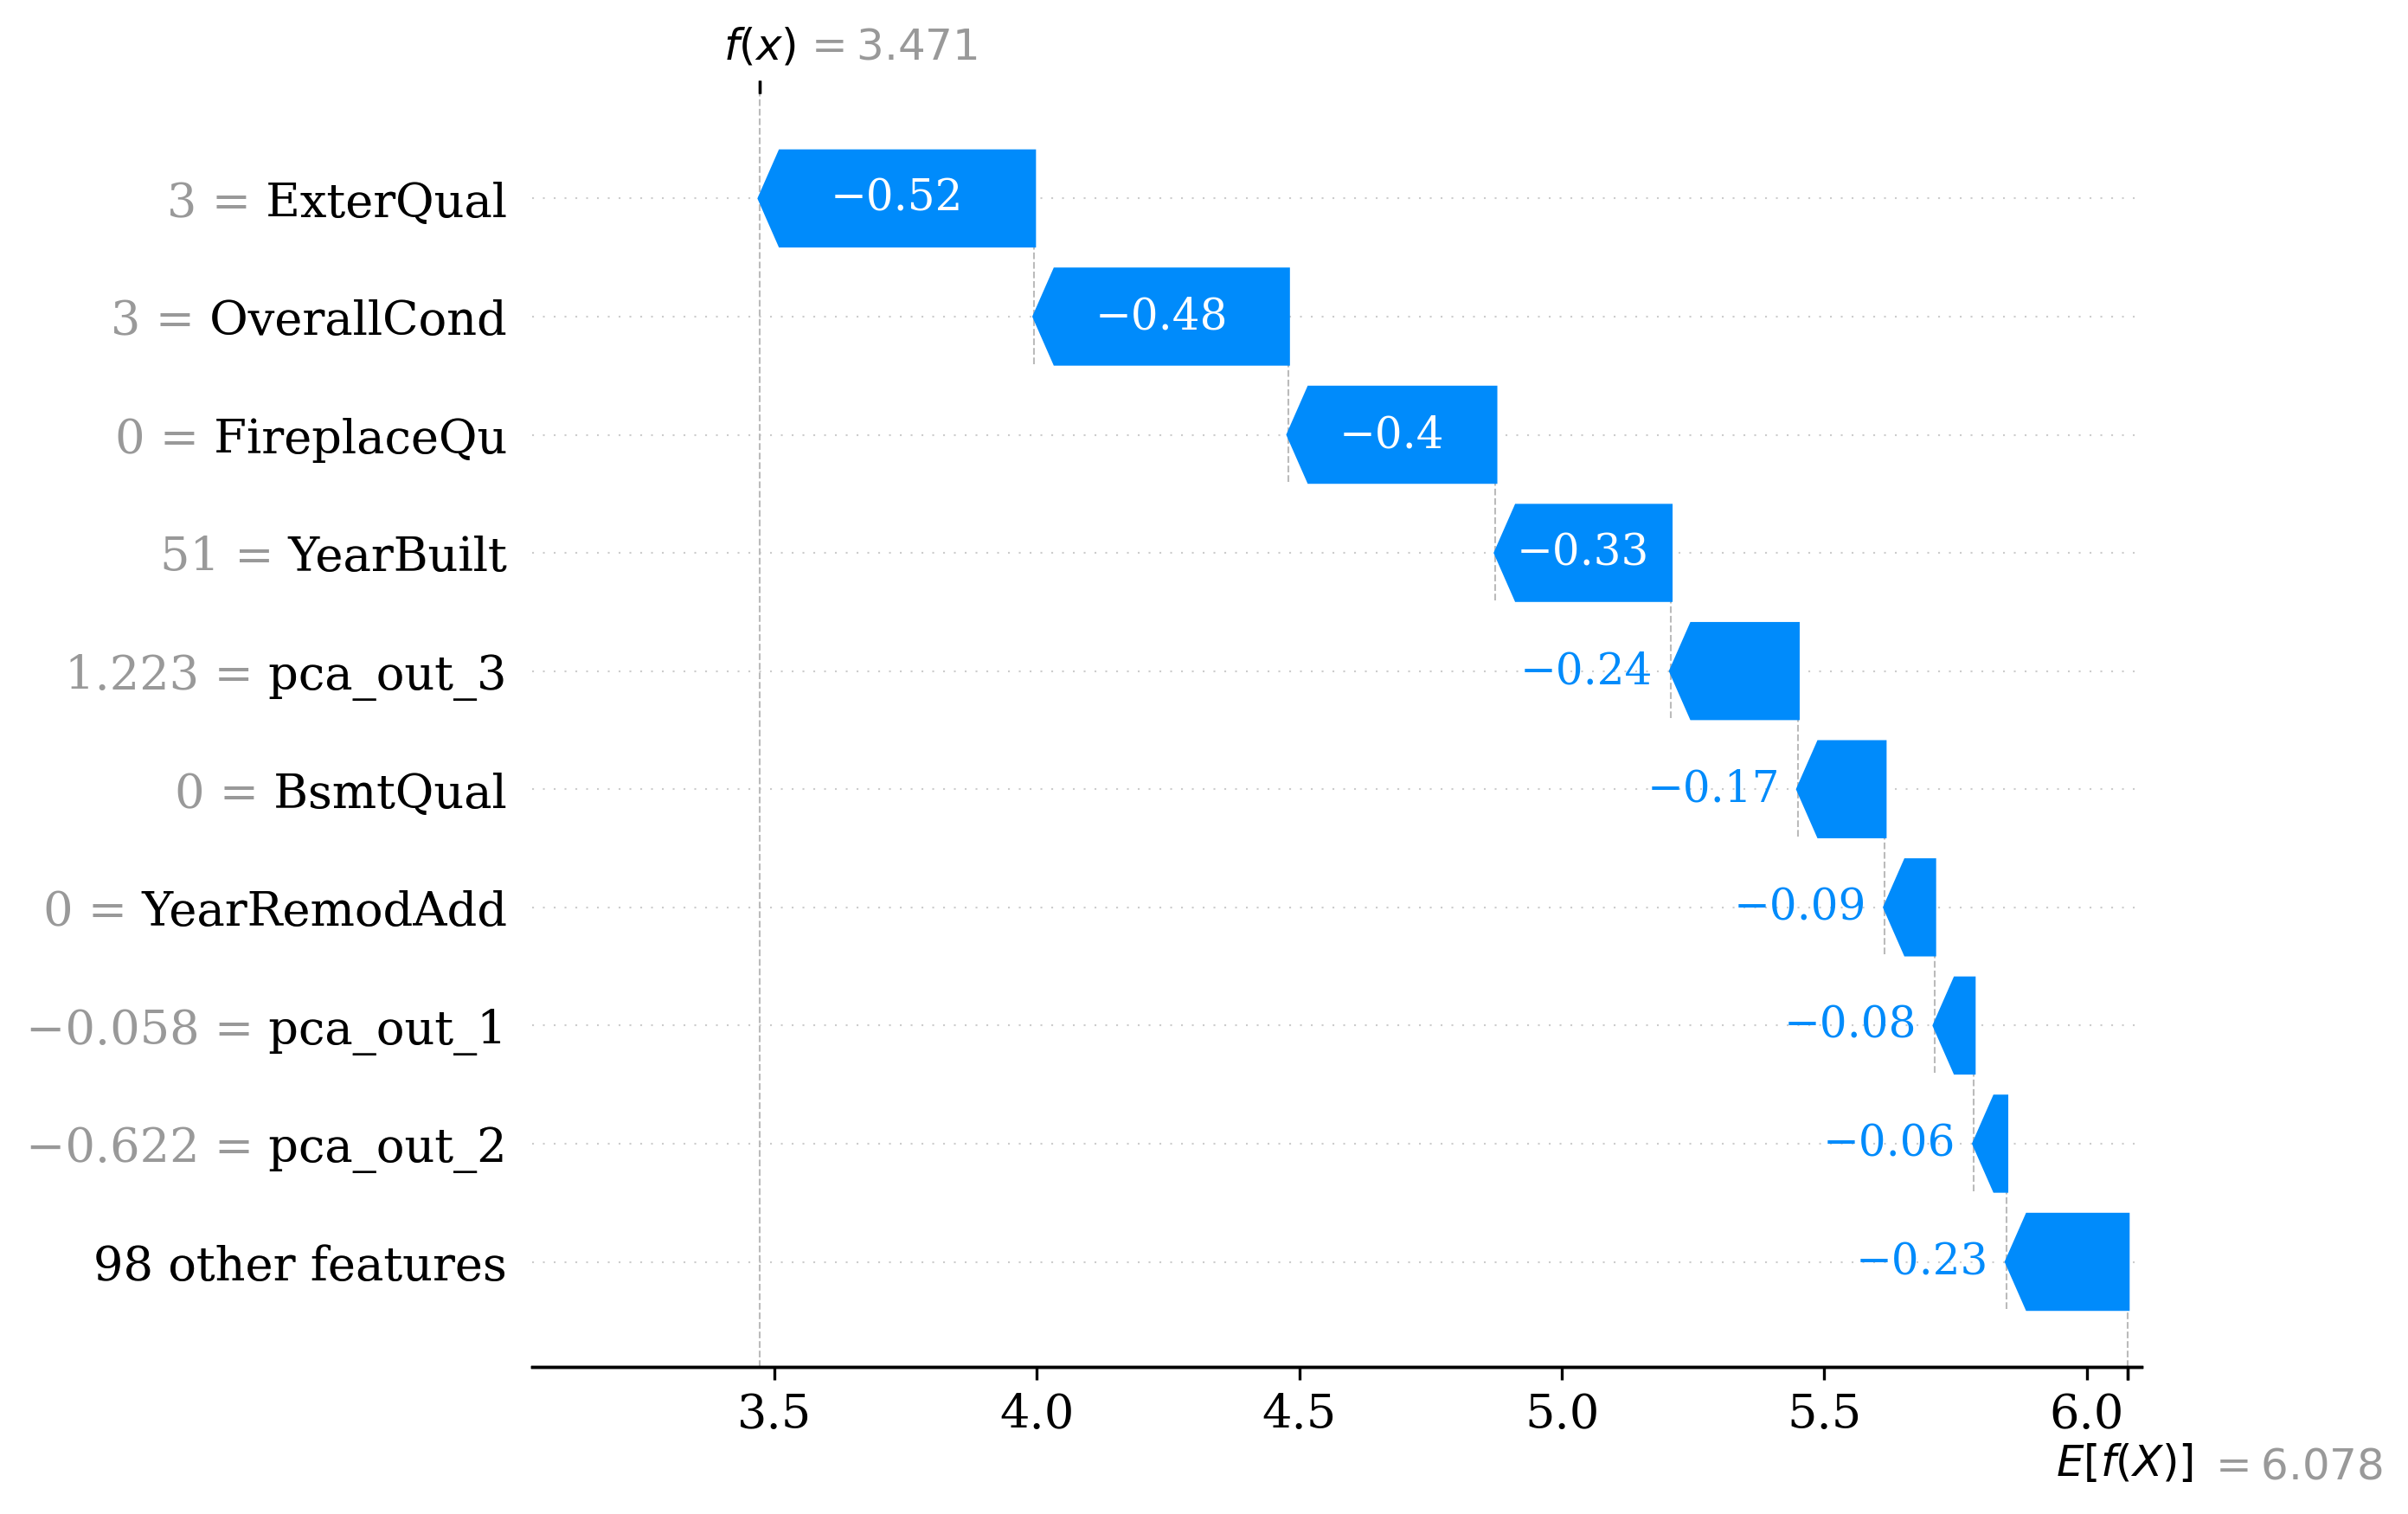
\includegraphics[width = 0.5 \textwidth]{shap-local-3.png}}
    \caption{SHAP - Feature contributions to the prediction}
    \label{fig:shap-local-3}
\end{figure}

Fig.~\ref{fig:shap-summary} shows how different values for each feature affect Shapley values. 
It implies that external quality is the most important attribute 
for overall quality, which is quite reasonable for housing market. The wider a variable's
different values are divided in terms of Shapley values, the more important the feature
is for the model. Hence, external quality, built year, and fireplace quality provide
the strongest signals to predict overall quality.
\begin{figure}[htbp]
    \centerline{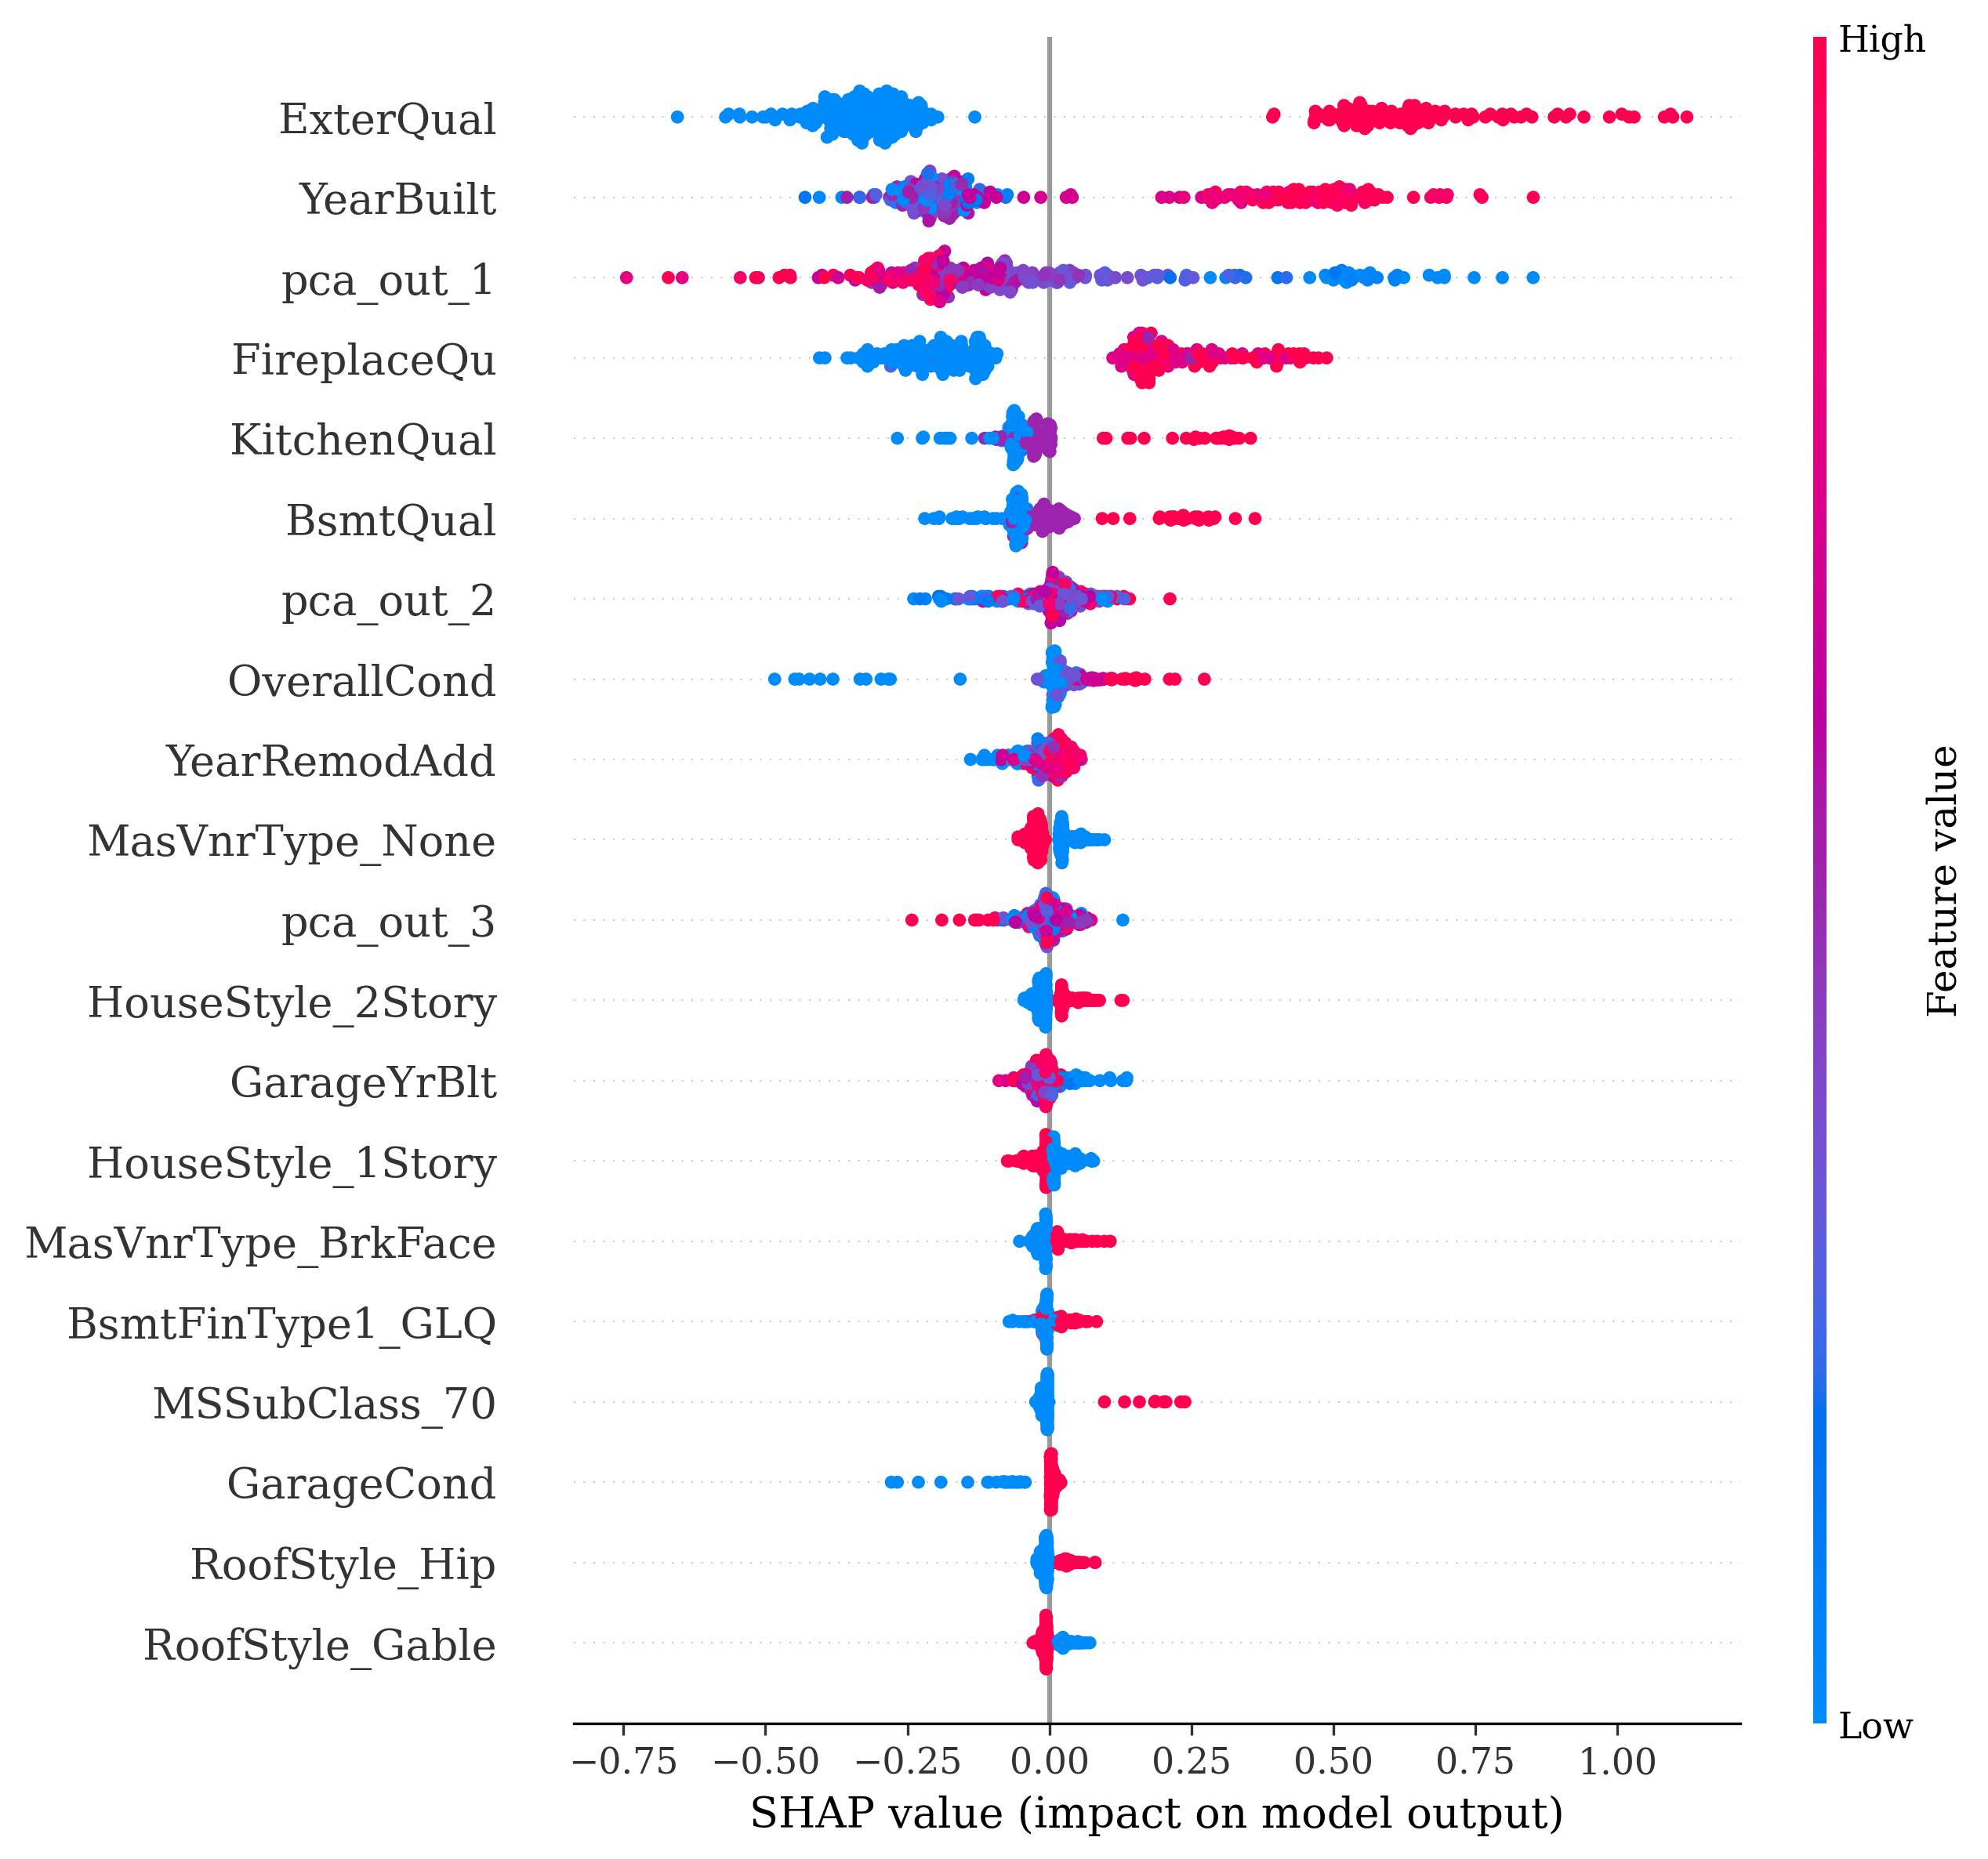
\includegraphics[width = 0.5 \textwidth]{shap-summary.png}}
    \caption{SHAP Summary}
    \label{fig:shap-summary}
\end{figure}

\section{Conclusion}

In this paper, we analyzed Ames Housing Dataset and trained a regression model 
to predict overall quality of the houses. We leveraged PCA and SHAP methods
for dimensionality reduction and feature selection respectively. We demonstrated that
SHAP method provides reasonable global and local explanations for the random forest
regressor trained.

\bibliographystyle{IEEEtran}
\bibliography{bibliography.bib}

\end{document}
